\section{Radiation Effects}
\newcommand{\letunit}{\unit{MeV/(mg/cm$^2$)}}

The plot shows the Single-Event-Upset (SEU) cross section for two devices in terms of the Linear Energy Transfer (LET) value of particles traversing the device. 

LET is a measure of the amount of energy deposited by an ionising particle when passing through a material. This depends on both the particle and the material, in addition to depending on the energy of the particle. In general, particles which are more energetic will produce fewer ionisations due to them having a shorter interaction time with the material. The opposite is true for less energetic particles. However, for very low energies, the particle may completely stop and not cause ionisations. 

In the case of memory devices, where information is stored in bits, which depend on the electronic state of a component and are binary in nature, an ionisation can "flip" a bit, making it go from one binary state to the other, completely altering the stored data. 

These curves show the cross section of these bit-flipping events on each device in terms of the LET of the ionising particle that may cause it.

Device 1 has a higher SEU cross-section for higher LET values than Device 2, but falls quicker to 0 when reducing LET. This means that for higher LET values, Device 1 will suffer more SEU than Device 2. However, for smaller values of LET (LET $\lesssim$9\letunit), Device 1 has a lower SEU cross-section (less likelihood of corruption) than Device 2. In fact, the SEU cross-section for Device 1 falls to 0 at around 5\letunit, whereas this happens to Device 2 at around 1\letunit. This shows that for LET values of 0-5\letunit, Device 2 will get SEU events, but not Device 1. This is what makes Device 1 more suitable for LEO satellites, because particles cosmic radiation reaching Low-Earth Orbit is more likely to have smaller LET values \cite{LEO}, thus making it valuable to have a small SEU cross-section for those than for high-LET particles.

Taking Device 1 now, and assuming a substrate layer of 70\unit{\textmu m} of Si and a fluence of 10$^7$\unit{ions/cm$^2$}, we can calculate what the energy of the Kr ions is after passing through the substrate. Using LISE++ \cite{lise}, it is possible to compute the energy loss of a \ce{^{82}Kr} beam at 768\unit{MeV} in silicon. LISE++ integrates the path of the beam using the values tabulated in SRIM \cite{srim}. With this, the energy loss is 593\unit{MeV} after 70\unit{\textmu m} of Si substrate. Therefore, 175\unit{MeV} remain when arriving at the memory.

Now, the LET of \ce{^{82}Kr} in Si at 175\unit{MeV} has to be obtained. This can also be taken from SRIM by considering that LET $\approx \frac{\d E}{\d x}$ for Kr. The LET of \ce{^{82}Kr} in Si at 175\unit{MeV} according to SRIM is 40.89\letunit. 

Now, it is only necessary to use:
\begin{equation}
    \label{eq:SEU}
    \sigma_{SEU} = \frac{N_{err}}{\Phi_{ion}N_{bit}}
\end{equation} to estimate the number of errors in the die. Reading from the given graph that the SEU cross-section for 41\letunit is $\sigma_{SEU} = 2.5\E{-11}\unit{cm$^2$/bit}$ and knowing that the memory contains $2048^3\unit{bits}$, it is then easy to calculate the expected number of errors:
\begin{displaymath}
    \label{eq:errors}
    N_{err} = \sigma_{SEU}\cdot\Phi_{ion}\cdot N_{bit} = 2.5\E{-11}\unit{cm$^2$/bit}\times10^7\unit{ions/cm$^2$}\times2048^3\unit{bits} = 2.15\E{6}.
\end{displaymath}

If the substrate had a variation of $\pm30\unit{\textmu m}$ from the thickness stated before, it would affect the number of errors, as it will affect the LET of the Kr beam when reaching the memory. Repeating the calculations done before, but for a $40\unit{\textmu m}$- and a $100\unit{\textmu m}$-thick substrate, the Kr beam energies after the substrate are:
\begin{center}
    \begin{tabular}{l@{ = }l}
        E(40\unit{\textmu m})  & 453.6\unit{MeV},\\
        E(100\unit{\textmu m}) & 0\unit{MeV}.
    \end{tabular}
\end{center}    
The beam will not penetrate the $100\unit{\textmu m}$-thick substrate, as its range at 768\unit{MeV} is 93.8\unit{\textmu m}. Plotting the LET values obtained from SRIM for this energy range, we obtain the curve shown in \autoref{fig:letenergy}. In the figure, it can be seen that the maximum value of LET is around the one obtained for the nominal thickness of 70\unit{\textmu m}, which corresponds to around 41\letunit. From the graph given in the question, we can see that all LET values under 41\letunit\ correspond to SEU cross-sections smaller than that of 41\letunit.

This means that the maximum SEU cross-section happens for a thickness of 70\unit{\textmu m}, and having different thicknesses in the given range only decreases this cross-section. Therefore, the number of expected errors should decrease if that much variation is present in the substrate thickness.

For energies over around 175\unit{MeV}, where the maximum LET happens, LET only varies by around 5 units. This decrease will only vary the cross-section within the same order of magnitude, therefore not affecting the final number of errors by much. However, for lower energies (thicker substrates), the LET drops rapidly. It is only below a LET of 10\letunit, however, that the change in cross section spans a different order of magnitude. This will happen only for the thickest of substrates, at thicknesses over 90\unit{\textmu m}. 
\newpage

Assuming a uniform distribution of imperfections from 40 to 100\unit{\textmu m}, thicknesses of 90\unit{\textmu m} or more will correspond to 16.7\% of the surface of the substrate. Due to the rapid fall of the cross-section below this, and the fact that energies over 10\unit{MeV} will correspond to approximately the same SEU cross-section, we can say that the number of errors expected when this imperfect thinning is considered will be 83.3\% of that obtained with a properly performed thinning, therefore: $$\boxed{N'_{err} \approx 0.833 N_{err} = 1.79\E{6}}$$

\begin{figure}[H]
    \centering
     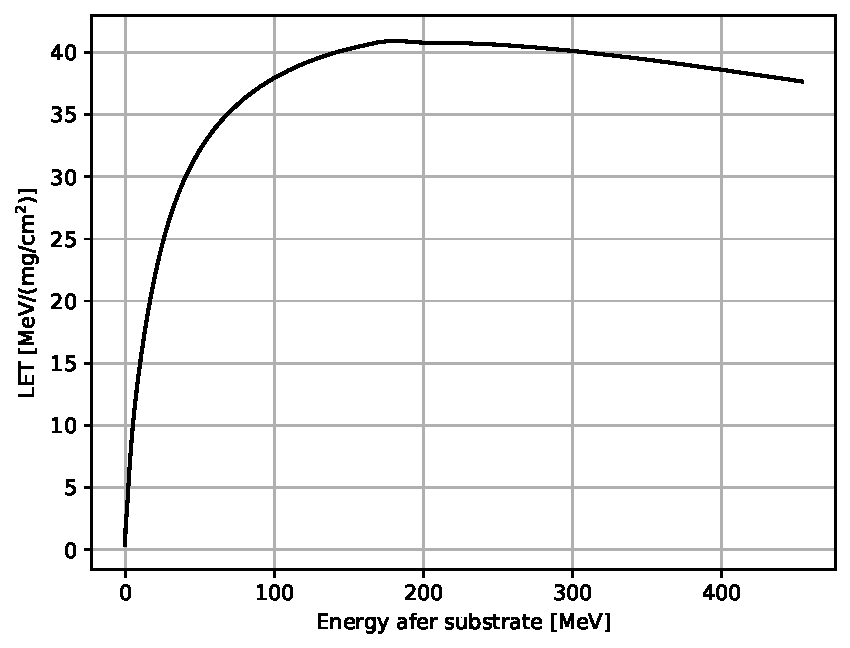
\includegraphics[width=\textwidth]{Kr_let.pdf}
     \caption{LET values for \ce{^{82}Kr} impinging on Si for different energy values, corresponding to a range of substrate thicknesses from 40 to 100\unit{\textmu m}. Values taken from SRIM \cite{srim}.} 
     \label{fig:letenergy}
 \end{figure}
